\chapter{Assignment A: Geographic and Cartesian Coordinates}
The main objective of the assignment is to understand the two commonly used coordinate frames for satellite-based positioning and grasp the transformations between the two coordinate frames. 

\section{Theory}
According to~\cite{misra2006global}, the transformation from the ellipsoidal coordiante frame $(\phi,\ \lambda,\ h)$ to the earth-centered, earth-fixed (ECEF) Cartesian coordinate frame $(x,\ y,\ z)$ can be computed as follows:
\begin{align}
	N &= \frac{a^2}{(1-e^2sin^2{\phi})^{\frac{1}{2}}} \\
	\left[\begin{matrix}
		x \\
		y \\
		z \\
	\end{matrix}\right] &= \left[\begin{matrix}
	(N+h) cos(\phi)cos(\lambda) \\
	(N+h) cos(\phi)sin(\lambda) \\
	(N(1-e^2)+h)sin(\phi) \\
	\end{matrix}\right] 
\end{align}
where, $a$ is the semi-major axis of ellipsoid ($6378137.0$ m), $e$ is the eccentricity of the ellipsoid calculated by $e^2=2f-f^2$ with $f$ being the flattening ($\frac{1}{298.257223563}$). This transformation can be computed directly.

The backward transformation from the ECEF to the ellipsoidal coordinate frame is given by:
\begin{align}
	p &= \sqrt{x^2+y^2}\\
\left[
	\begin{matrix}
	\phi \\
	\lambda \\
	h \\
	\end{matrix}
\right] &= \left[
	\begin{matrix}
	atan(\frac{z}{p(1-e^2\frac{N}{N+h})}) \\
	atan(\frac{y}{x}) \\
	\frac{p}{cos(\phi)}-N \\
	\end{matrix}
\right]
\label{eq:1.1}
\end{align}
As can be seen~\eqref{eq:1.1}, the $h$ and $\phi$ correlate with each other, which means it can only be solved iteratively. 

\section{Tasks}
\begin{itemize}
	\item Implement a \textsc{Matlab} function for conversion from Latitude, Longitude, and Height to X, Y, and Z (in WGS84), and vice versa.
	\item Test with positions selected from the internet.
	\item Benchmark the results with results converted by the KMSTrans\footnote{\url{http://valdemar.kms.dk/trf/}} program.
\end{itemize}
\section{Code}
%\textcolor{red}{TODO: comment useless code. add necessary explanantion.}
Complementary functions: \\
\textbf{deg2rad: conversion from degree to radian}:
\lstinputlisting{../../assignment/utils/deg2rad.m}
\textbf{rad2deg: conversion from radian to degree}:
\lstinputlisting{../../assignment/utils/rad2deg.m}
\textbf{llhtoCartesian: conversion from latitide, longitude, altitude to Cartesian coordiantes}:
\lstinputlisting{../../assignment/utils/llhtoCartesian.m}
\textbf{cartesian2llh: conversion from Cartesian coordiantes to latitide, longitude, altitude}:
\lstinputlisting{../../assignment/utils/cartesian2llh.m}
\newpage
\lstinputlisting{../../assignment/ex1/ex1_coordinate_transformation.m}

\section{Experiments}
\subsection{Simple Test}
\subsubsection{Setup}
In this simple test, I manually selected several points among which there is one point representing the DTU 101, one point located on the equator, one point in the North pole and one in the South pole. Meanwhile, in order to validate the correctness given the inputs contain negative values, the fourth point contains negative values for latitude, longitude. Below is a table listing the four sample points.
\begin{table}[h]
	\centering
	\caption{Test cases}
	\label{tb1:test_cases}
	\begin{tabular}{c|c}
		\hline
		\textbf{ID} & \textbf{\{lati, longi, alti\}} \\ \hline
		1     &  \{55.78575300466123,12.525384183973078,40\}   \\ \hline
		2     & \{0,12.525384183973078,40\}     \\ \hline
		3 	  & \{90,0,40\} \\ \hline
		4	  & \{-90,-15,40\} \\ \hline
	\end{tabular}
\end{table}
\subsubsection{Result}
\begin{table}[h]
	\centering
	\caption{Backward Results}
	\label{tb2:btest_results}
	\begin{tabular}{c|c|c}
		\hline
		\textbf{$LLA$} & \textbf{$LLA$} by KMSTrans & \textbf{$RMS$} with KMSTrans \\ \hline
		\{55.7858, 12.5254, 40\}  & \{55.5626, 12.3355, 40\}   &  0.1692  \\ \hline
		\{0, 12.5254, 40\}  & \{0, 12.3355, 40\}   &  0.1096  \\ \hline
		\{90, 0, 40\}  & \{90.1478, 0, 40\}   &  0.0853  \\ \hline
		\{-90, -15, 40\}  & \{\textcolor{red}{N/A}\footnote{KMSTrans does not support this point.}\}   &  \textcolor{red}{N/A}  \\ \hline
	\end{tabular}
\end{table}
\begin{table}[h]
	\centering
	\caption{Backward Results}
	\label{tb3:fbtest}
	\begin{tabular}{c|c|c}
		\hline
		\textbf{Original $LLA$} & \textbf{Reconstructed $LLA$} & \textbf{$RMS$} \\ \hline
		\{55.7858, 12.5254, 40\}  & \{55.7858, 12.5254, 40\}   &  $2.1508e^{-09}$  \\ \hline
		\{0, 12.5254, 40\}  & \{0, 12.5254, 40\}   &  $5.377e^{-10}$  \\ \hline
		\{90, 0, 40\}  & \{90, 0, 40\}   &  0  \\ \hline
		\{-90, -15, 40\}  & \{-90, -15, 40\} &  $1.0256e^{-15}$ \\ \hline
	\end{tabular}
\end{table}
The forward result is shown in the following Table~\ref{tb1:ftest_results} where the first column lists the transformed $XYZ$ values, the second column lists the results from the KMSTrans website, the third column lists the error between the computed values and the results from the KMSTrans website in terms of Root-Mean-Squares $RMS$. \\
The backward result is shown in the Table~\ref{tb2:btest_results}, where the first column lists the re-computed values for latitude, longitude, altitude $LLA$, the second column lists the results from the KMSTrans website, the last column lists the error between the re-computed values and the refereed values from KMSTrans for latitude, longitude, altitude in terms of Root-Mean-Squares $RMS$.
\noindent% <-- important
\begin{sidewaystable}
%\begin{sidewaystable}[htbp]
\centering
\caption{Forward Results}
\label{tb1:ftest_results}
	\small
	\setlength\tabcolsep{2pt}
\begin{tabular}{c|c|c}	
	\hline
	\textbf{$XYZ$} & \textbf{$XYZ$} by KMSTrans & \textbf{$RMS$ with KMSTrans} \\ \hline
	\{3509064.2531, 779572.0321, 5251099.25\}  & \{3509064.253, 779572.032, 5251099.25\}   &  $8.1650e^{-05}$  \\ \hline
	\{6226376.5177, 1383248.822, 0\}  & \{6226376.518, 1383248.822, 0.00\}   &  $1.7321e^{-04}$  \\ \hline
	\{3.9186e-10, 0, 6356792.3142\}  & \{0, 0, 6356792.31\}   &  $0.0024$  \\ \hline
	\{3.7851e-10, -1.0142e-10, -6356792.3142\}  & \{\textcolor{red}{N/A}\footnote{KMSTrans does not support negative latitude, longitude inputs.} \}   &  \textcolor{red}{N/A}  \\ \hline
\end{tabular}
\end{sidewaystable}
A further test is done to evaluate the accuracy of the backward transformation: with given $LLA$, firstly do the forward transformation and then do the backward transformation, then take the difference. Theoretically, the reconstructed result should be the same as the original values.
The real result is shown in Table~\ref{tb3:fbtest}.
\subsection{Brute-force Test}
In order to do more brute force tests conveniently, a \textsc{Matlab} GUI\footnote{Code is not attached here since there are a lot of GUI related codes.} is designed and shown in Fig~\ref{fig:gui}. Latitude, longitude, and altitude can be arbitrarily selected simply by sliding corresponding sliders. Transformation results will be shown once the "\textbf{Calculate}" button is pushed down. KMSTrans result (if available) can be automatically accessed by click "\textbf{web check}" button. \\
By playing with this GUI, I did a brute-force test. Generally speaking, if KMSTrans result is achievable, the results are similar with a small difference.
\begin{figure}[h]
	\centering
	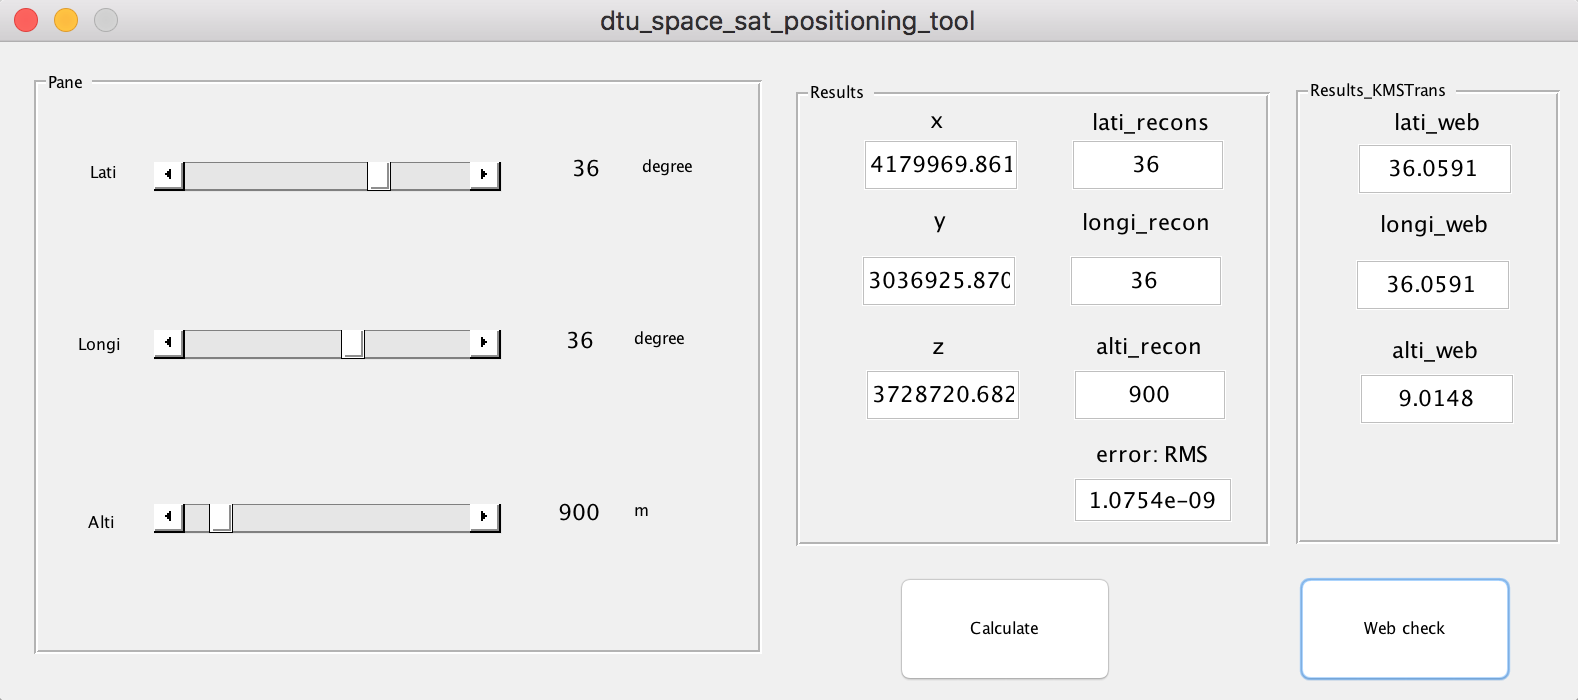
\includegraphics[width=\textwidth]{figures/gui.png}
	\caption{Snapshot of the designed GUI.}
	\label{fig:gui}
\end{figure}
\subsection{Conclusion}
Though various tests of my program, I believe that this program can correctly compute the coordinate transformation between the ECEF coordinate frame and the ellipsoidal coordinate frame. 